\section {Oszillatoren}
\subsection {Definition und Klassifikation von Oszillatoren \normalfont{\small{(Skript S.6-2)}}} 
\raggedright

Oszillatoren werden in zwei Hauptgruppen unterteilt:
\begin{compactitem}
    \item \textbf{Abgestimmte} Oszillatoren aus einem Verstärker und einem Frequenz bestimmenden Newtzwerk, die in \textbf{positiver} Rückkopplung betrieben werden.
    \item \textbf{Nichtabgestimmte} oder schaltende Oszillatoren bestehen dagegen aus einem Schaltelement mit mindestens zwei stabilen Zuständen (\textbf{Multivibrator}) und einem Integrator oder Tiefpassfilter, welches zwischen den Zuständen des Schaltelementes umgeladen wird. Die Umladezeit des Integrators ist hier Frequenz bestimmend während die Amplitude üblicherweise durch die Pegel des Schaltelementes gegeben ist.
\end{compactitem}
 
\centering
\begin{figure}[h!]
  \centering
  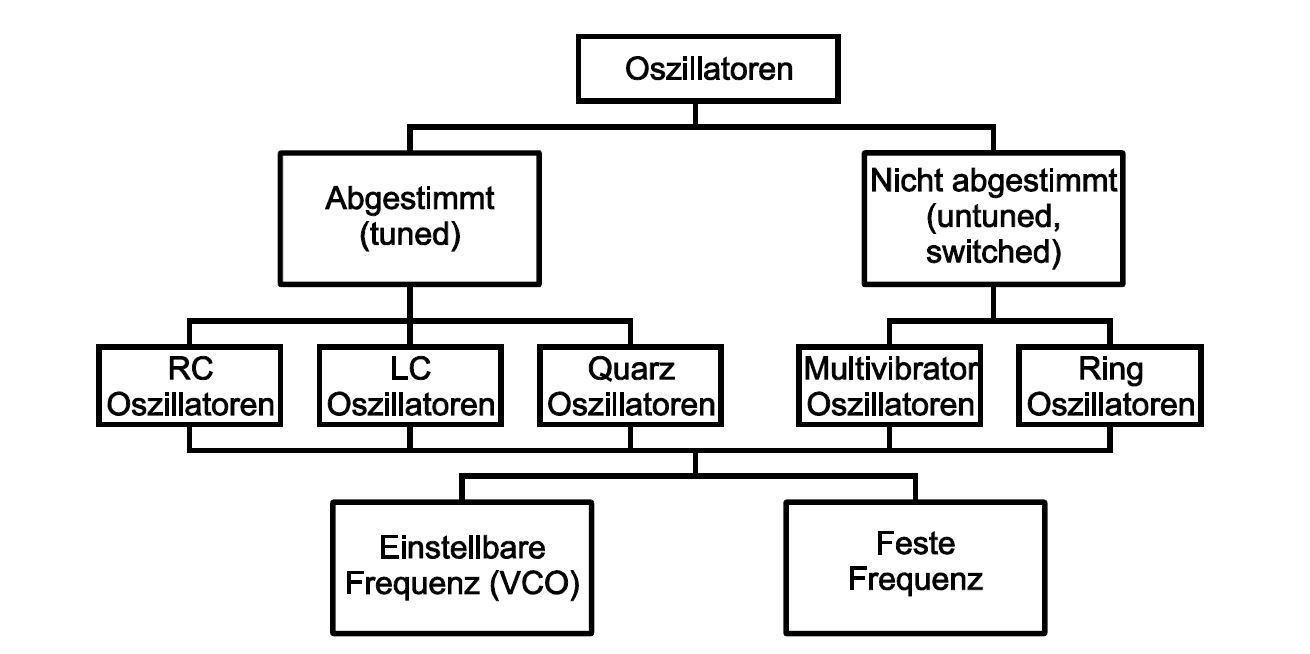
\includegraphics[width=0.8\textwidth]{images/Klassifikation_Oszillatortypen}
  \subcaption*{Klassifikation von Oszillatortypen}
\end{figure}

\FloatBarrier
\subsection{Oszillatorgrundprinzipien\normalfont{(Skript S.6-4)}}
\subsubsection{Die Rückkopplungsschleife (Feedback Loop) bei abgestimmten Oszillatoren}
\begin{figure}[h!]
	% minipage mit (Blind-)Text
	\begin{minipage}{0.3\textwidth} 
	  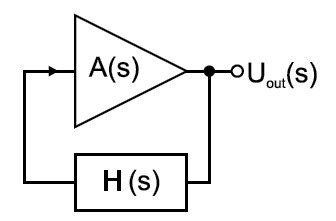
\includegraphics[width=1.0\textwidth]{images/Blockdiagramm_Oszillator}
	  \subcaption*{Blockdiagramm eines Oszillators}
	% \label{Text}
	\end{minipage}
	\begin{minipage}{0.4\textwidth}
	  \begin{equation*}
        \text{\textbullet }A_cl(s) =\frac{A_(s)}{1-A(s) \cdot H(s)} = \frac{A(s)}{1-T(s)}
      \end{equation*}
      \begin{compactitem}
        \item Schleifenverstärkung: $T(s)$\\
        \item Für die Oszillations- oder Schwingbedingung gilt: $T(s)=1$\\
        \item Für das Anschwingen gilt: $T(s)>1$\\ 
      \end{compactitem}
	\end{minipage}
\end{figure}
\raggedright
Die Schwingbedingung ist im Normalfall für genau eine Kreisfrequenz $\omega _0$ erfüllt. Man       spricht von Amplituden- und Phasenbedingung, die gleichzeitig bei $\omega _0$ efüllt sein müssen.

\FloatBarrier
\subsubsection{Amplitudenstabilisierung}
Die Schleifenverstärkung ist eine Funktion der Signalamplitude (nichtlinearer Effekt). Für anwachsenden Amplitude wird die Verstärkung kleiner. 
\begin{figure}[h!]
	% minipage mit (Blind-)Text
	\begin{minipage}{0.4\textwidth} 
	  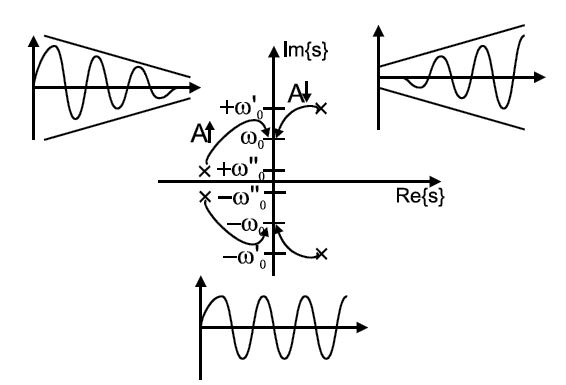
\includegraphics[width=1\textwidth]{images/Pollage_Regelung}
	  \subcaption*{Regelung der Pollage durch amplitudenabhängige Vertärkung}
	\end{minipage}
	\begin{minipage}{0.5\textwidth}
      \begin{compactenum}
        \item Anfangszustand: $T(s)=1$ (Pol befindet sich in rechter s-Halbene)
        \item Signalamplitude steigt exponentiell an.
        \item dadurch wird $T(s)$ reduziert
        \item dadurch werden Pole nach imag.-Achse verschoben (grenzstabil)
        \item falls Pol in inke s-Halbebene gelangt geschiet das umgekehrte
        \item dadurch werden Pole auf Achse gehalten
      \end{compactenum}
	\end{minipage}
\end{figure}

\FloatBarrier
\subsection{Abgestimmte Oszillatoren\normalfont{\small{(Skript S.6-7)}}}
\subsubsection{LC-Oszillatoren}
\begin{figure}[h!]
	% minipage mit (Blind-)Text
	\begin{minipage}{0.3\textwidth} 
	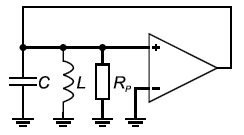
\includegraphics[width=1\textwidth]{images/LC-Oszillator}
	%\subcaption*{Regelung der Pollage durch amplitudenabhängige Vertärkung}
	\end{minipage}
	\begin{minipage}{0.6\textwidth}
      \begin{compactitem}
        \item Trankonduktanz-Verstärker liefert einen zur Eingangsspannung proportionalen Strom
        \item Rückkopplungsnetzwerk: LC-Resonator (Prinzip gilt auch für Serieresonator) 
        \item Schwingbedingung ist bei Resonanzfrequenz des Schwingkreises erfüllt.
        \item höhere Oszillationsfrequenzen möglich als mit RC-Netzwerk
        \item Einsatzgebiet: 1-10 MHz
      \end{compactitem}
       \begin{equation*} 
        \begin{split} 
          \omega_0=\frac{1}{\sqrt{LC}}
        \end{split} 
      \end{equation*}
	\end{minipage}
\end{figure}

\FloatBarrier
\subsubsection{Colpitts-Ozsillator}
\begin{figure}[h!]
	% minipage mit (Blind-)Text
	\begin{minipage}{0.3\textwidth} 
	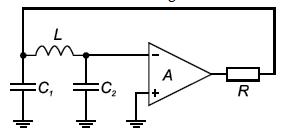
\includegraphics[width=1.1\textwidth]{images/Colpitts-Oszillator}
	\end{minipage}
	\begin{minipage}{0.6\textwidth}
      \begin{compactitem}
        \item Rückkopplungsnetzwerk: $\pi$-Netzwerk\\
      \end{compactitem}
      \begin{equation*} 
        \begin{split} 
           &T(s) = \frac{-A}{1+sR(C_1+C_2)+s^2LC_2+s^3RLC_1C_2}\\\\
           &\omega _0 = \frac{1}{\sqrt{L\frac{C_1 C_2}{C_1+C_2}}}\\\\
           &A =\frac{C_2}{C_1} \quad \quad \text{beim Anschwingen gilt:} \quad \quad A \geq\frac{C_2}{C_1} \\
           &\text{(A = Amplitude)} \\\\
        \end{split} 
      \end{equation*}
	\end{minipage}
\end{figure}

\FloatBarrier
\subsubsection{Quarz-Oszillator\normalfont{\small{(Skript S.6-8)}}}
\begin{figure}[h!]
	% minipage mit (Blind-)Text
	\begin{minipage}{0.3\textwidth} 
	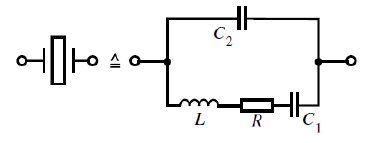
\includegraphics[width=1\textwidth]{images/Ersatzschaltbild_Schwingquarz}
	%\subcaption*{Regelung der Pollage durch amplitudenabhängige Vertärkung}
	\end{minipage}
	\begin{minipage}{0.6\textwidth}
	   Durch anlegen eine Wechselspannung an den Quarz, erhält man eine (bwz. mehrere) Resonsanzfrequenz(en).
       Eigenschaften von Schwingkreisen mit Quarz:
      \begin{compactitem}
        \item sehr temperaturstabil
        \item hohe Güte
        \item hohe Stabilität
        \item Typische Fehlertoleranz ($\frac{\Delta f}{f}$): +/- 20ppm (steigt jedoch quadratisch mit der Abweichung von der optimalen Temperatur (bei Uhrenquarz 25$^\circ$C)) $\rightarrow$ $\quad-0.04ppm/^\circ \text{C}^2$ (typ)\\
        $\frac{\Delta f}{f}=10^(-(^6))...10^(-^(1^(0)))=$
        \item Anschwingbedingung: $g_m \geq R_s\cdot4\omega_0^2C_0 ^2+\frac{4}{R_p}+\frac{1}{R_0}$
        \begin{compactitem}
          \item Es gilt: $ C_0 = C_p+C_1C_2/(C_1+C2)$
        \end{compactitem} 
      \end{compactitem} 
	\end{minipage}
	% minipage mit (Blind-)Text
	\begin{minipage}{0.3\textwidth} 
	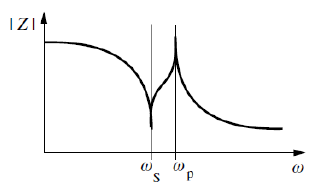
\includegraphics[width=1.0\textwidth]{images/Impedanz(Frequenz)_Schwingquarz}
	%\subcaption*{Regelung der Pollage durch amplitudenabhängige Vertärkung}
	\end{minipage}
	\begin{minipage}{0.6\textwidth}
      %\raggedright
      \vspace{0.5cm}
      Bei der Impedanz eines Schwingquarzes sieht man zwei wesentliche Eigenschaften:
      \begin{compactitem}
        \item zwei Resonanzfrequenzen: Serien- $(Im\{Z(\omega)\}=0)$ und Prallelresonanz $(Im\{Z(\omega)\}=\infty)$
        \item Impedanz ist weitgehend kapazitiv. Induktiv im Bereich:\\ $(\omega_s < \omega < \omega_p)$\\\\ 
      \end{compactitem}
      \begin{equation*} 
        \begin{split} 
         & Z (\omega)=\frac{s^2+\omega _s ^2}{sC_p(s^2+\omega_p ^2)} \quad \text{für } Z(s) = jX(\omega): \quad X(\omega)=-\frac{1}{\omega C_p}\cdot \frac{\omega^2-\omega_s ^2}{\omega^2-\omega_p ^2}\\\\
        \end{split} 
      \end{equation*}
	\end{minipage}
\end{figure}

\FloatBarrier
\subsection{Nichtabgestimmte Oszillatoren\normalfont{\small{(Skript S.6-10)}}}
\subsubsection{Multivibrator-Oszillatoren}
Beim Multivibrator wird der Verstärker durch einen Schmitt-Trigger (Komperator mit Hysterese) ersetzt. Als Frequenzbestimmendes Element wird ein RC-Netzwerk verwendet. Die Hysteresefunktion lässt sich dann ausnutzen, um einen Oszillator zu entwerfen. Das RC-Netzwerk als Rückkopplung dient als Tiefpass welcher eine grobe Annäherung eines Integrator darstellt.
\begin{figure}[h!]
	% minipage mit (Blind-)Text
	\begin{minipage}{0.3\textwidth} 
	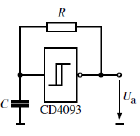
\includegraphics[width=0.7\textwidth]{images/Multivibrator_Komp}
	%\subcaption*{Regelung der Pollage durch amplitudenabhängige Vertärkung}
	\end{minipage}
	\begin{minipage}{0.6\textwidth}
      \begin{compactitem}
        \item max. Komperator Ausgangsspannung:\quad $L_+=V_+$
        \item min. Komperator Ausgnagsspannung:\quad $L_-=V_-$
        \item obere Umschaltschwelle: \quad $V_{TH}=\beta\cdot L_+$
        \item untere Umschaltschwelle: \quad $V_{TL}=\beta\cdot L_-$
        \item Teilungsfaktor: $\beta$\\\\
       \end{compactitem}
      \begin{equation*} 
        \begin{split} 
          &f_{osc}=\frac{1}{T} \quad \text{mit} \quad T=\tau \cdot ln \frac{(\beta L_- - L_+)(\beta L_+ - L_-)}{(\beta L_+ - L_+)(\beta L_- - L_-)}\\\\
          & \text{für} \quad   L_+=L_-: \quad  T=2\tau \cdotln\frac{\beta+1}{\beta-1}\\\\
        \end{split} 
      \end{equation*}
	\end{minipage}
\end{figure}

\FloatBarrier
\paragraph{Geschalteter Oszillator LM555}
Der LM555 ist ein fertiger IC welcher  mit einem Schmitt-Trigger und dessen Hysterese und exterenen RC-Beschaltung arbeiteite.
\begin{figure}[h!]
	\begin{minipage}{0.5\textwidth} 
	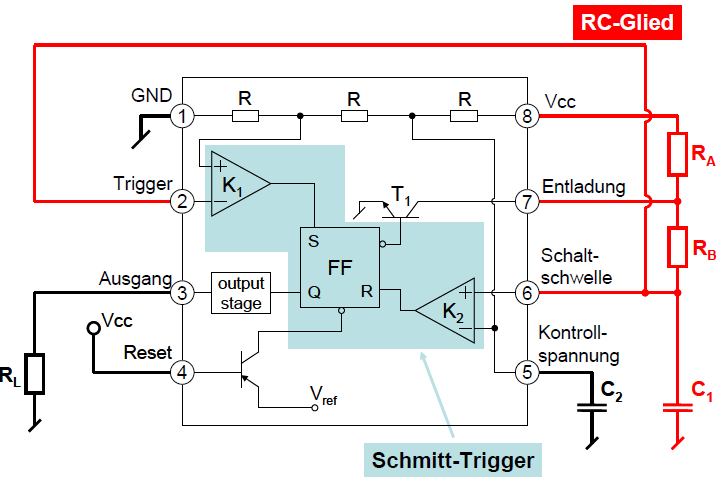
\includegraphics[width=1\textwidth]{images/LM555}
	%\subcaption*{Regelung der Pollage durch amplitudenabhängige Vertärkung}
	\end{minipage}
	\begin{minipage}{0.4\textwidth}
	  \begin{compactitem}
        \item Vorteil:
        \begin{compactitem}
           \item $f_{osc}$ ist nur von $R_a, R_B, C_1$ abhängig, nicht von der  Betriebsspannung
        \end{compactitem}
        \item Nachteile:
        \begin{compactitem}
           \item kleine $f_{osc}$
           \item Duty Cycle ist durch unterschiedliche Auf- und Entladezeiten normalerweise asymmetrisch.\\\
        \end{compactitem}
      \end{compactitem}
      \begin{listliketab}
    \begin{tabular}{Llll}
           & Ladezeit:             & $t_1=0.693\cdot(R_A+R_B)C$    \\
           & Entladezeit:          & $t_2=0.693\cdot R_B \cdot C$   \\
           &  Frequenz:             & $f=\frac{1}{T}=\frac{1.44}{(R_A+2\cdot R_B)C}$    \\
    \end{tabular}
\end{listliketab}
	\end{minipage}
\end{figure}

\FloatBarrier
\subsubsection{Ringozsillator\normalfont{\small{(Skript S.6-15)}}}
Beim Ringoszillator wird eine ungerade Anzahl Inverter aneinander gereit. Die Frequenz ensteht durch die totale Verzögerung, welche sich aus den einzelnen Verzögerungen der Inverter ergibt.
\begin{figure}[h!]
	\begin{minipage}{0.4\textwidth} 
	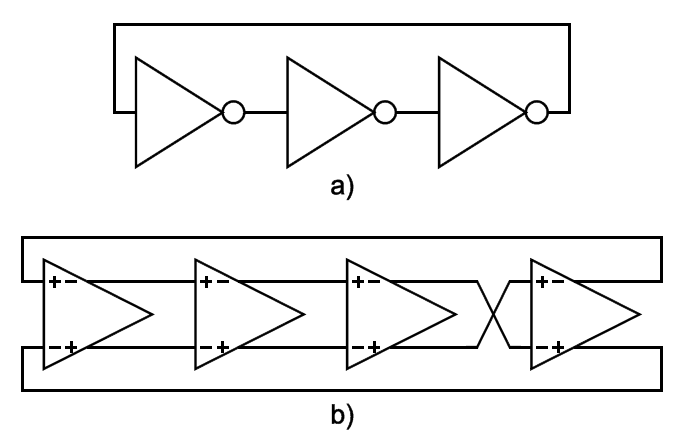
\includegraphics[width=1\textwidth]{images/Ring_Osc}
	\subcaption*{Ringoszillator mit a) CMOS-Invertern und b) differentiellen Invertern}
	\begin{equation*} 
        \begin{split} 
          f_{osc} =\frac{1}{2n\cdot t_g} \quad \quad \Delta\varphi =\frac{180^\circ}{2n}   \\\\
        \end{split} 
      \end{equation*}
	\end{minipage}
	\begin{minipage}{0.5\textwidth}
	  \begin{compactitem}
        \item Vorteil:
        \begin{compactitem}
           \item hohe $f_{osc}$ 
        \end{compactitem}
        \item Nachteile:
        \begin{compactitem}
           \item $f_{osc}$ ungenau
        \end{compactitem}
        \item Einsatz:
        \begin{compactitem}
           \item Prozesscharakterisierung
           \item Als gesteuerte Oszillatoren in PLL's\\
        \end{compactitem}
        \item Verzögerung ist Abhängig von der Versorungsspannung
        \item Verzögerung erhöht sich, wenn der Ausgang kapazitiv belastet wird (\"fan-out\")
        \item $n$: Anzahl Inverter
        \item $t_g$: Verzögerung pro Inverter
        \item $\Delta\varphi$: Phansenverschiebung
      \end{compactitem}
	\end{minipage}
\end{figure}

\FloatBarrier
\subsection{Spannungsgesteuerte Oszillatoren (VCO)\normalfont{\small{(Skript S.6-17)}}}
Mathematische Beschreibung siehe Kapitel \ref{Kap.VCO}.
Das Ziel ist es, bekannte Oszillatortopologien so zu nutzen, dass man sie mit einer Spannung oder einem Strom steuern kann. Dafür gibt es folgende Methoden (Siehe Beispiele ab S.6-20 in Skript):

\FloatBarrier
\subsubsection{FET im Anlaufgebiet}
FET's weisen im Anlaufgebiet lineare Anstiege auf, wodurch sie in diesem Bereich als steuerbare Wiederstände eingesetzt werden können.

\FloatBarrier
\subsubsection{Binär geschaltete Elemente}
Da der lineare Werterbereich eines FET's nicht sehr gross ist, werden sie oft als Schalter gebrucht. Dabei wird ein Netzwerk mit R,L,C aufgebaut welche durch die FET's je nach wunsch dazugeschalten werden können. Die FET's nhemen also die Zustände $"$on$"$ oder $"$off$"$ ein. Es handelt sich um eine digitale Ansteuerung. Oft werden C's parallet geschlten, da man diese dann addieren kann und man so mit einem Binärwort gut ansteuern kann. VCO's dessen Frequenz sich mit einem Binärwort in diskreten Schritten einstellen lassen, nennt man $"$Digital Controlled Oscillator (DCO)$"$.

\FloatBarrier
\subsubsection{Diode im Sperrbereich}
Wenn man eine Diode im Sperrbereich betreibt, entsteht eine Sperrschichtkapazität. Diese ist von der DC-Sperrspannung $V_SP$ abhängig. Man hat also einen spannungsgesteuerten Kondensator, den man in einem Schwingkreis einsetzen kann.
\begin{equation*} 
  C_D(V_{SP})=\frac{C_0}{(1+\frac{V_{SP}}{\Phi})^m}
\end{equation*)

\FloatBarrier
\subsubsection{Referenzspannung beim Multivibrator (LM555)}
Durch Veränderung der Schaltschwelle eines Multivibrators lässt sich die Auf- und Entladezeit des Fre-quenz bestimmenden Kondensators variieren. Leider wird durch Manipulation der Schaltschwelle beim Schmitt-Trigger nur die Dauer einer Halbperiode beein-flusst, so dass die Frequenzvariation nur zum "Preis" einer Tastverhältnisvariation erhältlich ist.

\FloatBarrier
\subsubsection{Delay-Interpolation}
\begin{figure}[h!]
	\begin{minipage}{0.3\textwidth} 
      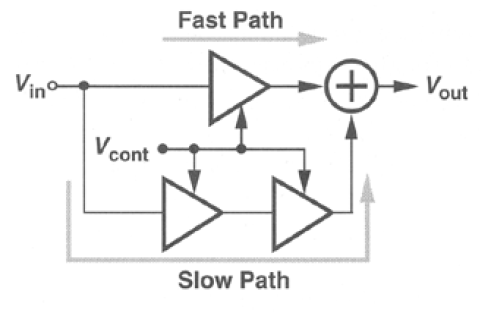
\includegraphics[width=1\textwidth]{images/Fast_Path}
    \end{minipage}
    \begin{minipage}{0.6\textwidth} 
       Bei Ringoszillatoren kann bei differenziellen Invertern die effektive Anzahl Inverter durch Ändern des Schaltstromes zwischen zwei Extremen geändert werden.
       \begin{equation*} 
         f_{min} =\frac{1}{2n_{max}\cdot t_g} \quad \text{und} \quad f_{max} =\frac{1}{2n_{min}\cdot t_g}   \\\\
       \end{equation*}
    \end{minipage}
\end{figure}

